% THIS IS SIGPROC-SP.TEX - VERSION 3.1
% WORKS WITH V3.2SP OF ACM_PROC_ARTICLE-SP.CLS
% APRIL 2009
%
% It is an example file showing how to use the 'acm_proc_article-sp.cls' V3.2SP
% LaTeX2e document class file for Conference Proceedings submissions.
% ----------------------------------------------------------------------------------------------------------------
% This .tex file (and associated .cls V3.2SP) *DOES NOT* produce:
%       1) The Permission Statement
%       2) The Conference (location) Info information
%       3) The Copyright Line with ACM data
%       4) Page numbering
% ---------------------------------------------------------------------------------------------------------------
% It is an example which *does* use the .bib file (from which the .bbl file
% is produced).
% REMEMBER HOWEVER: After having produced the .bbl file,
% and prior to final submission,
% you need to 'insert'  your .bbl file into your source .tex file so as to provide
% ONE 'self-contained' source file.
%
% Questions regarding SIGS should be sent to
% Adrienne Griscti ---> griscti@acm.org
%
% Questions/suggestions regarding the guidelines, .tex and .cls files, etc. to
% Gerald Murray ---> murray@hq.acm.org
%
% For tracking purposes - this is V3.1SP - APRIL 2009

\documentclass{acm_proc_article-sp}

\usepackage{url}
\usepackage{listings}
\usepackage{graphicx}
\usepackage{fixltx2e}
\usepackage{moreverb}
\usepackage{fancyvrb}
\usepackage{csvsimple}
\linespread{2}
\begin{document}

\numberofauthors{2} 
\author{
\alignauthor
Ivan Oropeza\\
       \affaddr{Dept. of Computer Science}\\
       \affaddr{University of Texas at Austin}\\
\alignauthor
William Xie\\
       \affaddr{Dept. of Computer Science}\\
       \affaddr{University of Texas at Austin}\\
}

\title{Hidden Markov Models vs. Maximum Entropy Markov Models}


\maketitle
\section{Introduction}
A frequent problem in many disciplines is the challenge to do sequence labelling. DNA sequencing, video semantic analysis, and Part-Of-Speech tagging are just some examples where sequence labelling is the underlying problem that needs to be solved~\cite{dnaEx, videoEx, nlpEx}. In Natural Language Processing (NLP), Part-Of-Speech (POS) or lexical category tagging is an important problem because it serves as a stepping stone into solving more complex problems such as semantic analysis of sentences. The typical techniques applied to this problem are Hidden Markov Models (HMM), Maximum Entropy Markov Models (MEMM), and Conditional Random Fields (CRF)~\cite{nlpBook}. While CRFs are considered to be the state-of-the-art in POS tagging we want to compare the performance of the other models, HMM and MEMM. This paper is structured in the following way: first we provide a brief description of the corpora used in this investigation. Then, we discuss some of the differences between HMMs and MEMMs. Next, we explain how the training process works specifically for POS tagging. Finally, we compare the performance of HMMs vs MEMMs under similar circumstances.

\section{Datasets}
In this investigation we use two corpora. The first one is the Wall Street Journal (WSJ) corpus. The WSJ corpus is a collection of 2,499 articles collected in a span of three years from the Wall Street Journal. It has approximately 3 million words and was tagged by using statistically-based methods. This corpus has a total of 82 possible tags~\cite{wsjCorpus}. Its range of topics is very narrow and thus it is reasonable to expect that the word choice distribution in the articles to be narrower than other corpora as well. Hence, we expect better performance when we test with this metric.

In addition to the WSJ corpus, we also use the Brown corpus. The Brown corpus is a manually tagged collection of 500 text documents sampled from 1961. It uses 36 POS tags and it is consolidated from various sources and from various topics such as fiction, press, and lore~\cite{brownCorpus}. Consequently, we expect that this corpus would represent a more general distribution on word choice than WSJ corpus. Therefore, we expect scores to be slightly lower than when using WSJ.

\begin{figure}[ht]
 \begin{Verbatim}[frame=single,framesep=5mm]
\[ He/PRP \]
tried/VBD to/TO ignore/VB 
\[ what/WP \]

\[ his/PRP\$ own/JJ common/JJ sense/NN \]
told/VBD 
\[ him/PRP \]
,/, but/CC 
\[ it/PRP \]

\[ was/VBD n't/RB possible/JJ \]
;/: ;/: 
\[ her/PRP$ motives/NNS \]
were/VBD too/RB blatant/JJ ./.
\end{Verbatim}
\caption{Example sentence from the Brown Corpus~\cite{brownCorpus} \label{brownExample}}
\end{figure}

\section{HMM vs. MEM,}
A HMM is generative model for the joint distribution of states and observations. It follows a Markov assumption. In other words, it is the assumption that restricts the transitions between states to be dependent only on the immediate past~\cite{nlpBook}. On the other hand, MEMM is discriminative since it models the conditional probability of the current state given the observation and the prior state. 

An MEMM is an enhancement on the Maximum Entropy model, also known as a multinomial regression model which in turn attempts to do classification by making the fewest number of assumptions. Figure \ref{hmmVmemm} shows pictorially the differences between both graphical models. The benefit of MEMMs over HMMs is that MEMMs are not limited to only modelling two aspects: the transition probabilities $P( S_i | S_{i-1} )$ and emission probabilities $P( O_i | S_i )$. Instead, MEMMs can integrate feature information from the observations in addition to the previous state knowledge in order to derive a more accurate prediction model. For example, capitalization often occurs with Nouns and specific suffixes such as "-ed" and "-ing" tend to be associated with Verbs are useful features that can not be modelled by an HMM but can be easily modelled by an MEMM. Moreover, this model does not restrict us to only analysing the current observation. It is entirely possible to have features that take observations that occur in the neighbourhood of the current observation~\cite{nlpBook}. Finally, the typical algorithm used to solve the decoding problem in an HMM can be trivially modified to solve the decoding problem in an MEMM without additional overhead~\cite{memmPaper}.

Another difference between HMM and MEMM is that MEMM is susceptible to the "label bias problem". This issue generally arises in two forms, differences in entropy in the states and uncertainty during testing. Whenever there are states with small entropy (fewer outgoing edges) then the observation will be less influential during the decoding process (the extreme case being when the state only has one outgoing edge). In POS tagging this takes the form of having observations that are abnormally more frequent in the dataset. The other source of label bias is during the decoding process. During training of the model
\begin{figure}[ht]
\centering
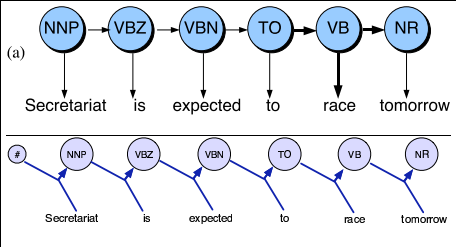
\includegraphics[width=80mm]{figures/memm.png}
\caption{Hidden Markov Model(top) and Maximum Entropy Markov Model(bottom)~\cite{nlpBook}. \label{hmmVmemm}}
\end{figure}

\section{Learning}
In POS tagging, training an HMM model in a supervised fashion reduces to a simple counting procedure~\cite{nlpBook}. In order to estimate $P( S_i | S_{i-1} )$ and $P( O_i | S_i )$, we can assume that our annotated corpus is a representative sample of the distribution we want to model, we can then define the latter quantities as follows:

$P( S_i | S_{i-1} ) \approx \hat{P}( S_i | S_{i-1} ) = C( S_i, S_{i-1} )/C( S_{i-1} )$

$P( O_i | S_i ) \approx \hat{P}( O_i | S_i ) = C( O_i, S_i )/C( S_i )$

where $\hat{P}$ is the probability with respect to the corpus and $C( O_i, S_i ), C( S_i, S_{i-1} )$, and $C( S_i )$ are the appropriate occurrence and co-occurrence of the observations and states.

However there is one additional issue that needs to be addressed before the model can be used for tagging, how should the model respond to words it did not encounter during training? If left unattended then $P( O_i | S_i ) = 0$. Consequently, Viterbi's algorithm will make incorrect decision during the decoding process. The technique we employ to address this issue is Laplace smoothing (also known as additive smoothing)~\cite{laplaceSmooth}. The general idea of this approach is that any every state will always have a small probability of producing a special symbol (in our case "<U>") and every time the model encounters an unknown word it will use $P( <U> | S_i )$ instead. The small probability is created by setting $C( <U>, S ) = 1$ and incrementing $C( S )$ for each state $S$ before calculating the emission probabilities and after calculating the transition probabilities.

XXXXXXXX MEMM Learning TODO XXXXXXXXXXX

\section{Experiment}
All our code is implemented in Python. Also, we enhance an general HMM python module with additive smoothing~\cite{hmmCode}. Moreover, we implement MEMM in its entirety including the learning and decoding process. 

XXXXXXXX MEMM BROKEN TODO XXXXXXXXXXX

The following tables show the results for both models when we execute our experiments using 20-fold cross-validation (train with 19 portions and test on 1). In addition to evaluating performance on the testing data we also evaluate the model's performance on the training data. Testing the model with training data will give us an idea of over fitting (how much generalizable is the model for this task) and testing with testing data will give us an idea of effectiveness of the system.

\begin{figure}[ht]
  \begin{tabular}{ l || c | c | c | c | c }
    \bfseries & \bfseries & \bfseries \overline{Sentence} & \bfseries \sigma Sentence & \bfseries \overline{Tag} & \bfseries \sigma Tag
    
    \csvreader[head to column names]{figures/hmmScores.csv}{}% use head of csv as column names
    {\\\hline\csvcoli&\csvcolii&\csvcoliii&\csvcoliv&\csvcolv&\csvcolvi}% specify your coloumns here
    \end{tabular}
    \caption{HMM percent scores (\%) for the Brown and WSJ corpora. The first column is the corpus used. The second column is the data used for evaluating the system. Four scores are reported: the average and stdev for the number of sentences correctly tagged and the average and stdev for the number of tags correctly labelled. The experiments \label{hmmScores}}
\end{figure}

Given that our implementation of MEMM performs considerably worse than expected (possibly caused by a bug or GIS is converging at a local maxima), we can not directly compare the performance of both models for POS tagging as we would have liked. Ideally, we would compare not only the overall performance of the models but also determine which POS tags had a boost in accuracy and also which ones decreased. From our intuition by adding features that help Noun or Verb tagging we should see an increase in performance for Noun and Verbs in MEMMs. 

Never the less, the literature shows that MEMM tend to outperform HMM in POS tagging. Brants reports that their HMM POS tagger reaches 96.46\% accuracy in the WSJ corpus while Denis and Sagot's MEMM tagger correctly tags sentences in WSJ 96.96\% of the time~\cite{memmAhmmResultsACL}. Figure ~\ref{allScores} shows the results for various experiments in POS tagging.

\begin{figure}[ht]
  \begin{tabular}{ l | c | c | c | c | r }
    \bfseries Corpus & \bfseries Model & \bfseries Accuracy & \bfseries Authors
    
    \csvreader[head to column names]{figures/otherResults.csv}{}% use head of csv as column names
    {\\\hline\csvcoli&\csvcolii&\csvcoliii&\csvcoliv}% specify your coloumns here
    \end{tabular}
    \caption{Accuracy results for various POS tagging experiments. The empty author cells represent our experiments \label{allScores}}
\end{figure}

\bibliographystyle{abbrv}
\bibliography{references}
\end{document}
